\section{收敛与计算成本}
\label{sec:qn-convergence}

前面各节展示了许多好现象，但例子都很小。于是要问：这些方法在什么条件下能保证什么？答案要分开说，因为不同的更新规则、线搜索和目标类型，对应的结论强弱不同。

全节的基本假设是：$f$二阶连续可微，存在$0<\mu\leq L$使$\mu\bm{I}\preceq\nabla^2f(\bm{x})\preceq L\bm{I}$对所有$\bm{x}$成立，$\bm{x}^\star$是唯一最优解。需要放宽时会明确说明。

\paragraph{一步下降与方向角}
先把线搜索的贡献算清楚。记$\theta^{(t)}$为$\bm{d}^{(t)}$与$-\bm{g}^{(t)}$的夹角，
\begin{equation}
 \cos\theta^{(t)}=\frac{-\langle\bm{g}^{(t)},\bm{d}^{(t)}\rangle}{\lVert\bm{g}^{(t)}\rVert_2\lVert\bm{d}^{(t)}\rVert_2}.
 \label{eq:qn-cos-theta}
\end{equation}
方向越接近负梯度，$\cos\theta^{(t)}$越接近$1$；方向几乎与梯度垂直时，它接近$0$，再好的步长也下降有限。

\begin{lemma}[Wolfe线搜索的一步下降]
\label{lem:qn-one-step}
设$\nabla f$是$L$-Lipschitz的，$\bm{d}^{(t)}$是下降方向，$\alpha^{(t)}$满足式~\eqref{eq:qn-wolfe}。则
\begin{equation}
 f(\bm{x}^{(t+1)})\leq f(\bm{x}^{(t)})-\frac{c_1(1-c_2)}{L}\cos^2\theta^{(t)}\lVert\bm{g}^{(t)}\rVert_2^2.
 \label{eq:qn-one-step}
\end{equation}
\end{lemma}

\begin{proof}
省略上标。由第二条Wolfe不等式和梯度的Lipschitz性，得到
\[
 (c_2-1)\langle\bm{g},\bm{d}\rangle\leq\langle\bm{g}^{+}-\bm{g},\bm{d}\rangle\leq\alpha L\lVert\bm{d}\rVert_2^2.
\]

这给出步长的下界：
\[
 \alpha\geq\frac{(1-c_2)\lvert\langle\bm{g},\bm{d}\rangle\rvert}{L\lVert\bm{d}\rVert_2^2}.
\]

把它代入第一条Wolfe不等式，并用式~\eqref{eq:qn-cos-theta}，得到
\[
 f(\bm{x}^{+})\leq f(\bm{x})-c_1\alpha\lvert\langle\bm{g},\bm{d}\rangle\rvert
 \leq f(\bm{x})-\frac{c_1(1-c_2)}{L}\cdot\frac{\langle\bm{g},\bm{d}\rangle^2}{\lVert\bm{d}\rVert_2^2},
\]
最后一个分式等于$\cos^2\theta\lVert\bm{g}\rVert_2^2$。
\end{proof}

把式~\eqref{eq:qn-one-step}对$t$求和，并用$f$有下界，就得到称为\term{Zoutendijk条件}（Zoutendijk condition）的结论$\sum_t\cos^2\theta^{(t)}\lVert\bm{g}^{(t)}\rVert_2^2<\infty$。所以只要$\cos\theta^{(t)}$不趋于零，梯度就要趋于零。全局收敛的问题变成：方向角能不能控制住？

\paragraph{BFGS的全局收敛}
BFGS的矩阵可能很差，方向可能很偏。下面的定理说，只要目标强凸，差的方向不可能一直出现。证明的工具是一个衡量矩阵“病态程度”的势函数，这也就是自校正的数学内容。

\begin{theorem}[BFGS在强凸目标上的全局收敛]
\label{thm:qn-bfgs-global}
设$f$满足本节的基本假设，$\bm{B}^{(0)}\succ\bm{0}$，步长满足Wolfe条件~\eqref{eq:qn-wolfe}，所有$\bm{g}^{(t)}\neq\bm{0}$。则BFGS的迭代点满足
\begin{equation}
 \lim_{t\to\infty}\bm{x}^{(t)}=\bm{x}^\star.
 \label{eq:qn-bfgs-global}
\end{equation}
\end{theorem}

\begin{proof}
由式~\eqref{eq:qn-wolfe-curvature}和定理~\ref{thm:qn-positive-definite}，所有$\bm{B}^{(t)}$正定。定义势函数
\[
 \psi(\bm{B})=\operatorname{tr}\bm{B}-\ln\det\bm{B}=\sum_{i=1}^n(\lambda_i-\ln\lambda_i),
\]
其中$\lambda_i$是$\bm{B}$的特征值。因为$\lambda-\ln\lambda\geq1$，所以$\psi(\bm{B})>0$。它同时惩罚过大和过小的特征值。

第一步，估计测量的尺度。省略上标，由式~\eqref{eq:qn-average-hessian}，并令$\bm{z}=\bar{\bm{H}}^{1/2}\bm{s}$，得到
\[
 \frac{\langle\bm{s},\bm{y}\rangle}{\langle\bm{s},\bm{s}\rangle}\geq\mu,\qquad
 \frac{\langle\bm{y},\bm{y}\rangle}{\langle\bm{s},\bm{y}\rangle}=\frac{\bm{z}^\top\bar{\bm{H}}\bm{z}}{\bm{z}^\top\bm{z}}\leq L.
\]

第二步，计算迹和行列式的变化。对式~\eqref{eq:qn-bfgs-direct}取迹，得到
\[
 \operatorname{tr}\bm{B}^{+}=\operatorname{tr}\bm{B}-\frac{\lVert\bm{B}\bm{s}\rVert_2^2}{\bm{s}^\top\bm{B}\bm{s}}+\frac{\lVert\bm{y}\rVert_2^2}{\langle\bm{s},\bm{y}\rangle}.
\]

行列式把$\bm{B}$提出来，写成
\[
 \det\bm{B}^{+}=\det\bm{B}\cdot\det\Bigl(\bm{I}-\frac{\bm{s}(\bm{B}\bm{s})^\top}{\bm{s}^\top\bm{B}\bm{s}}+\rho\,\bm{W}\bm{y}\bm{y}^\top\Bigr).
\]
括号内是$\bm{I}+\bm{U}\bm{C}^\top$的形式，其中$\bm{U}$的两列是$-\bm{s}/(\bm{s}^\top\bm{B}\bm{s})$与$\rho\bm{W}\bm{y}$，$\bm{C}$的两列是$\bm{B}\bm{s}$与$\bm{y}$。由行列式的恒等式（交换乘积因子，维数从$n$降到$2$），$\bm{I}+\bm{U}\bm{C}^\top$与$\bm{I}+\bm{C}^\top\bm{U}$的行列式相同。沿用第~\ref{sec:qn-dfp-bfgs}节的曲率比$\tau$，则
\[
 \bm{I}+\bm{C}^\top\bm{U}=\begin{bmatrix}0&1\\-\tau&1+\rho\,\bm{y}^\top\bm{W}\bm{y}\end{bmatrix},
\]
这个矩阵的行列式是$\tau$，因此
\[
 \det\bm{B}^{+}=\det\bm{B}\cdot\frac{\langle\bm{s},\bm{y}\rangle}{\bm{s}^\top\bm{B}\bm{s}}.
\]

第三步，用方向角重写。由$\bm{B}\bm{d}=-\bm{g}$和$\bm{s}=\alpha\bm{d}$，式~\eqref{eq:qn-cos-theta}的夹角满足
\[
 \cos\theta=\frac{\bm{s}^\top\bm{B}\bm{s}}{\lVert\bm{s}\rVert_2\lVert\bm{B}\bm{s}\rVert_2}.
\]

再引入三个比值：
\[
 q=\frac{\bm{s}^\top\bm{B}\bm{s}}{\langle\bm{s},\bm{s}\rangle},\qquad m_{\mathrm{c}}=\frac{\langle\bm{s},\bm{y}\rangle}{\langle\bm{s},\bm{s}\rangle},\qquad M_{\mathrm{c}}=\frac{\langle\bm{y},\bm{y}\rangle}{\langle\bm{s},\bm{y}\rangle}.
\]
于是迹和行列式公式中的两个量可以写成
\[
 \frac{\lVert\bm{B}\bm{s}\rVert_2^2}{\bm{s}^\top\bm{B}\bm{s}}=\frac{q}{\cos^2\theta},\qquad
 \frac{\langle\bm{s},\bm{y}\rangle}{\bm{s}^\top\bm{B}\bm{s}}=\frac{m_{\mathrm{c}}}{q}.
\]

把第二步的结果代入$\psi$，整理得到
\[
 \psi(\bm{B}^{+})=\psi(\bm{B})+(M_{\mathrm{c}}-\ln m_{\mathrm{c}}-1)
 +\Bigl[1-\frac{q}{\cos^2\theta}+\ln\frac{q}{\cos^2\theta}\Bigr]+\ln\cos^2\theta.
\]
方括号非正，因为$1-v+\ln v\leq0$对$v>0$成立。令$c=\max\{L-\ln\mu-1,\,1\}>0$，由第一步，
\[
 \psi(\bm{B}^{(t+1)})\leq\psi(\bm{B}^{(0)})+c(t+1)+\sum_{j=0}^{t}\ln\cos^2\theta^{(j)}.
\]

第四步，反证。设$\cos\theta^{(t)}\to0$，则存在$t_1$，当$j>t_1$时$\ln\cos^2\theta^{(j)}<-2c$。对$t>t_1$，上式右端不超过
\[
 \psi(\bm{B}^{(0)})+c(t+1)+\sum_{j\leq t_1}\ln\cos^2\theta^{(j)}-2c(t-t_1).
\]
它随$t$线性趋于$-\infty$，与$\psi>0$矛盾。所以存在$\delta>0$和子列使$\cos\theta^{(t)}\geq\delta$。

第五步，收敛。对引理~\ref{lem:qn-one-step}求和，得到Zoutendijk条件，所以沿这个子列$\lVert\bm{g}^{(t)}\rVert_2\to0$。第~\ref{chap:optimization}章的误差换算给出下面两个不等式：
\[
 f(\bm{x})-f^\star\leq\frac{\lVert\nabla f(\bm{x})\rVert_2^2}{2\mu},\qquad
 \frac{\mu}{2}\lVert\bm{x}-\bm{x}^\star\rVert_2^2\leq f(\bm{x})-f^\star.
\]
前一个说明沿子列$f(\bm{x}^{(t)})\to f^\star$。

$f(\bm{x}^{(t)})$单调，于是整个序列的目标值都收敛到$f^\star$。再由后一个不等式，迭代点收敛到$\bm{x}^\star$。
\end{proof}

用贯穿例的BFGS（$\bm{B}^{(0)}=\bm{I}$，精确线搜索）核对一下这个公式。三个矩阵的$\psi$值是
\[
 \begin{gathered}
 \psi(\bm{B}^{(0)})=2,\qquad\psi(\bm{B}^{(1)})=7.8-\ln5\approx6.191,\\
 \psi(\bm{B}^{(2)})=10-\ln16\approx7.227.
 \end{gathered}
\]

第一次更新$\cos\theta^{(0)}=1$、$q=1$，方括号与最后的对数都是零，增量全部来自尺度项。按定理证明中的记号，$M_{\mathrm{c}}=6.8$，$m_{\mathrm{c}}=5$，于是
\[
 \psi(\bm{B}^{(1)})-\psi(\bm{B}^{(0)})=6.8-\ln5-1\approx4.191.
\]

第二次更新的方向角满足$\cos^2\theta^{(1)}\approx0.735$，此时$q/\cos^2\theta^{(1)}=1$，方括号仍是零。尺度项是$3.2-\ln2.353-1\approx1.344$，而$\ln\cos^2\theta^{(1)}\approx-0.308$，两者之和与$\psi$的实际增量$1.036$一致。

定理的证明解释了自校正：$\psi$每一步至多增加一个常数，而每次方向偏得厉害都要付出$\ln\cos^2\theta$这一项的大幅减少，方向不可能一直偏。证明中的第二步用到了BFGS特有的迹和行列式公式，不能搬给DFP；我们也不声称DFP在Wolfe线搜索下有同样的结论，图~\ref{fig:qn-dfp-bfgs-scaling}(b)显示它确实可能很慢。

对一般非凸目标，没有类似的定理：已有构造性例子说明，即使线搜索满足Wolfe条件，BFGS也可能不收敛到驻点。实践中BFGS常常工作良好，但这不是定理所保证的。

\paragraph{局部收敛的刻画：Dennis--Moré条件}
全局收敛说的是终将到达，还要看到达的速度。称$\bm{x}^{(t)}\to\bm{x}^\star$是\term{超线性收敛}（superlinear convergence），如果
\begin{equation}
 \lim_{t\to\infty}\frac{\lVert\bm{x}^{(t+1)}-\bm{x}^\star\rVert_2}{\lVert\bm{x}^{(t)}-\bm{x}^\star\rVert_2}=0.
 \label{eq:qn-superlinear}
\end{equation}
Newton法靠的是矩阵趋于Hessian。拟牛顿矩阵一般并不趋于Hessian，超线性收敛却仍然可能发生。下面的定理说明，真正需要的只是沿步方向准确。

\begin{theorem}[Dennis--Moré特征]
\label{thm:qn-dennis-more}
设$f$二阶连续可微，$\bm{x}^{(t)}\to\bm{x}^\star$，$\bm{x}^\star$是驻点，$\bm{H}^\star=\nabla^2f(\bm{x}^\star)$正定。设对充分大的$t$，迭代取单位步长且方向$\bm{d}^{(t)}\neq\bm{0}$由$\bm{B}^{(t)}\bm{d}^{(t)}=-\bm{g}^{(t)}$确定。则序列超线性收敛，当且仅当
\begin{equation}
 \lim_{t\to\infty}\frac{\lVert(\bm{B}^{(t)}-\bm{H}^\star)\bm{d}^{(t)}\rVert_2}{\lVert\bm{d}^{(t)}\rVert_2}=0.
 \label{eq:qn-dennis-more}
\end{equation}
\end{theorem}

\begin{proof}
省略上标，把误差写成$\bm{e}=\bm{x}-\bm{x}^\star$、$\bm{e}^{+}=\bm{x}^{+}-\bm{x}^\star$。与式~\eqref{eq:qn-average-hessian}一样，梯度差等于平均Hessian乘$\bm{d}$。代入$\bm{g}=-\bm{B}\bm{d}$，得到关键等式
\[
 \bm{g}^{+}=(\bar{\bm{H}}-\bm{H}^\star)\bm{d}+(\bm{H}^\star-\bm{B})\bm{d}.
\]
因为$\bm{x}^{(t)}\to\bm{x}^\star$且Hessian连续，所以$\bar{\bm{H}}\to\bm{H}^\star$，第一项是$o(\lVert\bm{d}\rVert_2)$。

充分性：设式~\eqref{eq:qn-dennis-more}成立，则$\lVert\bm{g}^{+}\rVert_2=o(\lVert\bm{d}\rVert_2)$。在$\bm{x}^\star$附近，$\nabla^2f$的最小特征值不小于某个$\mu_{\star}>0$，所以
\[
 \lVert\bm{g}^{+}\rVert_2\geq\mu_{\star}\lVert\bm{e}^{+}\rVert_2.
\]

再由三角不等式，$\lVert\bm{d}\rVert_2$不超过两个误差的范数之和，于是
\[
 \lVert\bm{e}^{+}\rVert_2\leq o(1)\bigl(\lVert\bm{e}\rVert_2+\lVert\bm{e}^{+}\rVert_2\bigr).
\]
移项即得$\lVert\bm{e}^{+}\rVert_2=o(\lVert\bm{e}\rVert_2)$。

必要性：设序列超线性收敛。由三角不等式，$\lVert\bm{d}\rVert_2$不小于$\lVert\bm{e}\rVert_2-\lVert\bm{e}^{+}\rVert_2$，而$\lVert\bm{e}^{+}\rVert_2=o(\lVert\bm{e}\rVert_2)$，于是$\lVert\bm{e}\rVert_2=O(\lVert\bm{d}\rVert_2)$。

$\nabla f$在$\bm{x}^\star$处为零且连续可微，所以$\lVert\bm{g}^{+}\rVert_2$是$\lVert\bm{e}^{+}\rVert_2$的同阶小量，于是
\[
 \lVert\bm{g}^{+}\rVert_2=o(\lVert\bm{e}\rVert_2)=o(\lVert\bm{d}\rVert_2).
\]
由关键等式解出第二项，并用$\bar{\bm{H}}\to\bm{H}^\star$，得到式~\eqref{eq:qn-dennis-more}。
\end{proof}

式~\eqref{eq:qn-dennis-more}称为\term{Dennis--Moré条件}（Dennis--Moré condition）。它只比较矩阵在搜索方向上的作用，所以拟牛顿矩阵不必收敛到Hessian。图~\ref{fig:qn-rates}(b)印证了这一点：迭代结束时矩阵整体的误差约为$3\%$，沿步方向的误差约为$0.08\%$。

定理假设步长最终是$1$。满足式~\eqref{eq:qn-dennis-more}且$c_1<1/2$时，Wolfe线搜索最终确实接受单位步长，证明可查阅\scite{math-nocedal2006numerical}。这也是线搜索要优先试$\alpha=1$的理由：如果不试，或者试了又不接受，上面的超线性机制就用不上。

\paragraph{BFGS的超线性收敛}
完整记忆的BFGS确实满足Dennis--Moré条件，但需要更强的正则性。若$\bm{x}^{(t)}\to\bm{x}^\star$，$\bm{H}^\star$正定，$\nabla^2f$在$\bm{x}^\star$附近Lipschitz连续，且$\sum_t\lVert\bm{x}^{(t)}-\bm{x}^\star\rVert_2<\infty$，又有单位步长优先试探的线搜索，则BFGS超线性收敛。

证明要沿用定理~\ref{thm:qn-bfgs-global}的势函数并在$\bm{H}^\star$定义的坐标下估计，篇幅较长，读者可查阅\scite{math-nocedal2006numerical}。求和条件要求误差足够快地衰减，在定理~\ref{thm:qn-bfgs-global}的强凸条件下可以进一步证明它成立。Lipschitz条件的作用是控制$\bar{\bm{H}}^{(t)}$与$\bm{H}^\star$之差，使测量误差可以累加。

\begin{BookInlineFigure}
  \centering
  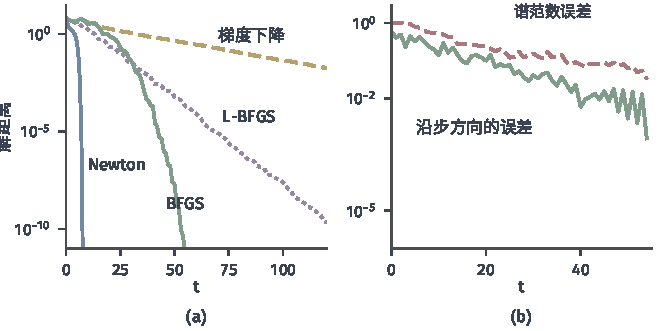
\includegraphics[width=112mm]{figures/05-optimization/02-smooth-optimization/matplotlib/qn-rates/figure.pdf}
  \caption{不同方法的局部速度，目标是$50$维的旋转$\ln\cosh$函数（$c_i$在$[0.1,100]$上对数等距，$\bm{x}^\star=\bm{0}$），强Wolfe线搜索。(a)解距离随迭代的变化：梯度下降（黄虚线）线性且慢，$r=5$的L-BFGS（紫点线）线性，BFGS（绿）后期斜率变陡，Newton法（蓝）最快。(b)BFGS的矩阵相对误差：红虚线是$\lVert\bm{B}^{(t)}-\bm{H}^\star\rVert_2/\lVert\bm{H}^\star\rVert_2$，绿线是Dennis--Moré比值$\lVert(\bm{B}^{(t)}-\bm{H}^\star)\bm{s}^{(t)}\rVert_2/(\lVert\bm{H}^\star\rVert_2\lVert\bm{s}^{(t)}\rVert_2)$。}
  \label{fig:qn-rates}
\end{BookInlineFigure}

\paragraph{SR1的局部结论}
SR1的结论需要不同的条件，第~\ref{sec:qn-sr1}节的定理只覆盖二次目标。对一般目标，已有的结果大致是：在$\bm{H}^\star$正定、分母保持远离零、步方向具有一致线性无关性质时，$\bm{B}^{(t)}$本身收敛到Hessian，配合信赖域可得到$n+1$步意义下的超线性收敛。这些条件比BFGS的条件更难事先验证，也不能换成Wolfe线搜索下的方向分析；相应证明见\scite{math-nocedal2006numerical}。

\paragraph{L-BFGS只保证线性收敛}
完整BFGS的超线性结论不能自动移给固定记忆的L-BFGS。超线性机制要求矩阵逐渐掌握沿步方向的曲率，而每轮重新从$\gamma\bm{I}$开始、只用$r$对向量的矩阵，无法累积足够的信息。下面的定理给出固定记忆下能证明的保证。

\begin{theorem}[L-BFGS的线性收敛]
\label{thm:qn-lbfgs-linear}
设$f$满足本节的基本假设，$t\geq1$时$\gamma^{(t)}$由式~\eqref{eq:qn-lbfgs-gamma}给出，$t=0$时取负梯度方向，记忆长度为$r$，步长满足Wolfe条件。令$T_{\mathrm{c}}=(n+r)L$，$\delta=(\mu/T_{\mathrm{c}})^{n+r}$。则
\begin{equation}
 f(\bm{x}^{(t+1)})-f^\star\leq\Bigl(1-\frac{2\mu c_1(1-c_2)\delta^2}{L}\Bigr)\bigl(f(\bm{x}^{(t)})-f^\star\bigr).
 \label{eq:qn-lbfgs-linear}
\end{equation}
\end{theorem}

\begin{proof}
设$\bm{B}_{[j]}=\bm{W}_{[j]}^{-1}$，它们由$\bm{B}_{[t-r]}=(1/\gamma^{(t)})\bm{I}$出发，按BFGS的直接形式更新$r$次。第一步，由定理~\ref{thm:qn-bfgs-global}证明中的尺度估计，$1/\gamma^{(t)}\in[\mu,L]$。

第二步，约束迹。式~\eqref{eq:qn-bfgs-direct}的修正中，减去的一项迹非负，加上的一项迹不超过$L$，于是
\[
 \operatorname{tr}\bm{B}_{[t]}\leq\frac{n}{\gamma^{(t)}}+rL\leq(n+r)L=T_{\mathrm{c}}.
\]
所以每个$\bm{B}_{[j]}$的最大特征值不超过$T_{\mathrm{c}}$。

第三步，约束行列式。由行列式公式和第一步，每次更新满足
\[
 \frac{\det\bm{B}_{[j+1]}}{\det\bm{B}_{[j]}}=\frac{\langle\bm{s},\bm{y}\rangle}{\bm{s}^\top\bm{B}_{[j]}\bm{s}}\geq\frac{\mu\lVert\bm{s}\rVert_2^2}{T_{\mathrm{c}}\lVert\bm{s}\rVert_2^2}=\frac{\mu}{T_{\mathrm{c}}}.
\]
连乘至多$r$次（窗口未满时次数更少，因$\mu/T_{\mathrm{c}}\leq1$，下界不变），并用$\det\bm{B}_{[t-r]}\geq\mu^n$，得到
\[
 \det\bm{B}^{(t)}\geq\mu^n\Bigl(\frac{\mu}{T_{\mathrm{c}}}\Bigr)^r.
\]

第四步，约束方向角。最小特征值至少是行列式除以另外$n-1$个特征值的上界，所以$\bm{B}^{(t)}$的条件数不超过
\[
 \frac{T_{\mathrm{c}}^{\,n}}{\det\bm{B}^{(t)}}\leq\Bigl(\frac{T_{\mathrm{c}}}{\mu}\Bigr)^{n+r}=\frac{1}{\delta}.
\]

由$\bm{d}=-\bm{W}\bm{g}$，方向角满足
\[
 \cos\theta^{(t)}=\frac{\bm{g}^\top\bm{W}\bm{g}}{\lVert\bm{g}\rVert_2\lVert\bm{W}\bm{g}\rVert_2}\geq\frac{\lambda_{\min}(\bm{W})}{\lambda_{\max}(\bm{W})}\geq\delta.
\]

第五步，代入引理~\ref{lem:qn-one-step}，并用第~\ref{chap:optimization}章的$\lVert\bm{g}\rVert_2^2\geq2\mu(f-f^\star)$，即得式~\eqref{eq:qn-lbfgs-linear}。
\end{proof}

定理的常数$\delta$随$n+r$指数变小，几乎没有定量价值。它的意义在于定性：固定记忆时，矩阵的条件数有界，因而线性收敛，且这个结论不依赖超线性的机制。图~\ref{fig:qn-rates}(a)中L-BFGS的直线正是线性收敛的样子，实际的速度远比定理的常数好。

\paragraph{各方法的保证}
下表汇总本节的结论，列出的是使结论成立的条件，并非全部的可行条件。

\begin{BookInlineTable}
  \centering
  \small
  \begin{tabular}{p{15mm}p{39mm}p{39mm}}
    \toprule
    方法 & 全局 & 局部\\
    \midrule
    BFGS & 强凸＋Wolfe：收敛（已证） & Hessian Lipschitz、误差可和：超线性\\
    DFP & 本章的势函数论证不适用 & 不作结论\\
    SR1 & 二次目标：至多$n+1$步（已证） & 分母与步方向条件＋信赖域：$n+1$步意义下超线性\\
    L-BFGS & 强凸＋Wolfe：线性收敛（已证） & 不保证超线性\\
    \bottomrule
  \end{tabular}
  \caption{拟牛顿方法的收敛保证汇总。}
  \label{tab:qn-guarantees}
\end{BookInlineTable}

\paragraph{计算成本}
比较成本要固定相同的精度，并把各项都算上。下表列出每一步除梯度外的开销，$n$是变量维数，$r$是记忆长度，线搜索的函数和梯度计算次数另算。

\begin{BookInlineTable}
  \centering
  \begin{tabular}{lll}
    \toprule
    方法 & 存储 & 方向与更新的乘法次数\\
    \midrule
    梯度下降 & $n$ & $n$\\
    L-BFGS & $2rn$ & $(4r+1)n$\\
    BFGS、DFP、SR1 & $n^2/2$ & 约$4n^2$\\
    Newton法 & $n^2/2$ & 约$n^3/3$，另加形成Hessian\\
    \bottomrule
  \end{tabular}
  \caption{每步除梯度以外的存储与运算，Newton法按Cholesky分解计。}
  \label{tab:qn-cost}
\end{BookInlineTable}

单步开销低的方法不一定总开销低，要乘上迭代数才能比较。图~\ref{fig:qn-rates}的目标取$n=50$，达到解距离$10^{-8}$需要的迭代数和方向运算量如表~\ref{tab:qn-experiment-cost}所示。

\begin{BookInlineTable}
  \centering
  \begin{tabular}{lrrr}
    \toprule
    方法 & 迭代数 & 每步方向运算 & 方向运算合计\\
    \midrule
    梯度下降 & $458$ & $50$ & $2.3\times10^{4}$\\
    L-BFGS（$r=5$） & $104$ & $1050$ & $1.1\times10^{5}$\\
    BFGS & $51$ & $1.0\times10^{4}$ & $5.1\times10^{5}$\\
    Newton法 & $8$ & $4.2\times10^{4}$ & $3.3\times10^{5}$\\
    \bottomrule
  \end{tabular}
  \caption{图~\ref{fig:qn-rates}的目标（$n=50$）上达到解距离$10^{-8}$的迭代数与方向运算量，不含梯度和Hessian的计算。}
  \label{tab:qn-experiment-cost}
\end{BookInlineTable}

这张表不能单独读。这个目标上一次梯度要做两次$50\times50$的矩阵乘法，约$5000$次运算，所以梯度下降实际花在梯度上的开销约为$2.3\times10^{6}$，远超方向运算本身。Newton法的Hessian开销未计入；在$n=50$时分解很便宜，$n$增大后三次方项才成为主要矛盾。比较的结论要在实际的$n$、梯度和Hessian成本下重新算。

实际选择大致如下：$n$不大、梯度贵、要高精度时用完整BFGS；$n$很大时用L-BFGS，代价是只有线性速度的保证；需要负曲率信息时用SR1配信赖域。
